\section{Study Area}
\label{sec:study_area}

The study encompasses \ntotal catchments with delineated watersheds across the Russian Federation, spanning latitudes \minlat--\maxlat and longitudes \minlon--\maxlon (Figure~\ref{fig:gauge_network}).
Catchment areas range from \minarea to \maxarea (median: \medianarea), with small-to-medium basins (100--10{,}000~km$^2$) comprising 60\% of the dataset.
Catchments are distributed across major drainage basins: the Volga (European Russia), Ob and Yenisei (Western and Central Siberia), Lena (Eastern Siberia), and Amur (Far East), plus smaller Arctic and Pacific coastal drainages.

The dataset spans K\"{o}ppen zones ET/Dfc (tundra/subarctic), Dfb (continental), and BSk (semi-arid steppe).
Mean annual precipitation is 350--1{,}100~mm/yr; mean annual temperature $-10$ to $+10$\textdegree C.
Snow cover persists 60--250+ days depending on latitude; permafrost ranges from absent in the south to continuous in northeastern Siberia.
These gradients drive contrasting hydrological regimes: snowmelt-dominated pulses in the permafrost zone versus baseflow-sustained flow in temperate forests (Sect.~\ref{sec:technical_validation}).

Elevations span 50--2{,}800~m, from lowland rivers draining to the Caspian and Arctic seas to mountain headwaters in the Caucasus, Altai, and Sayan ranges.
Boreal taiga dominates in the north (up to 95\% forest), while southern steppe catchments are predominantly agricultural (up to 85\% cropland); urban fraction reaches 35\% near major cities.
Soils vary from clay-rich Chernozems in agricultural lowlands to sandy Podzols under permafrost.

\begin{figure}[htbp]
\centering
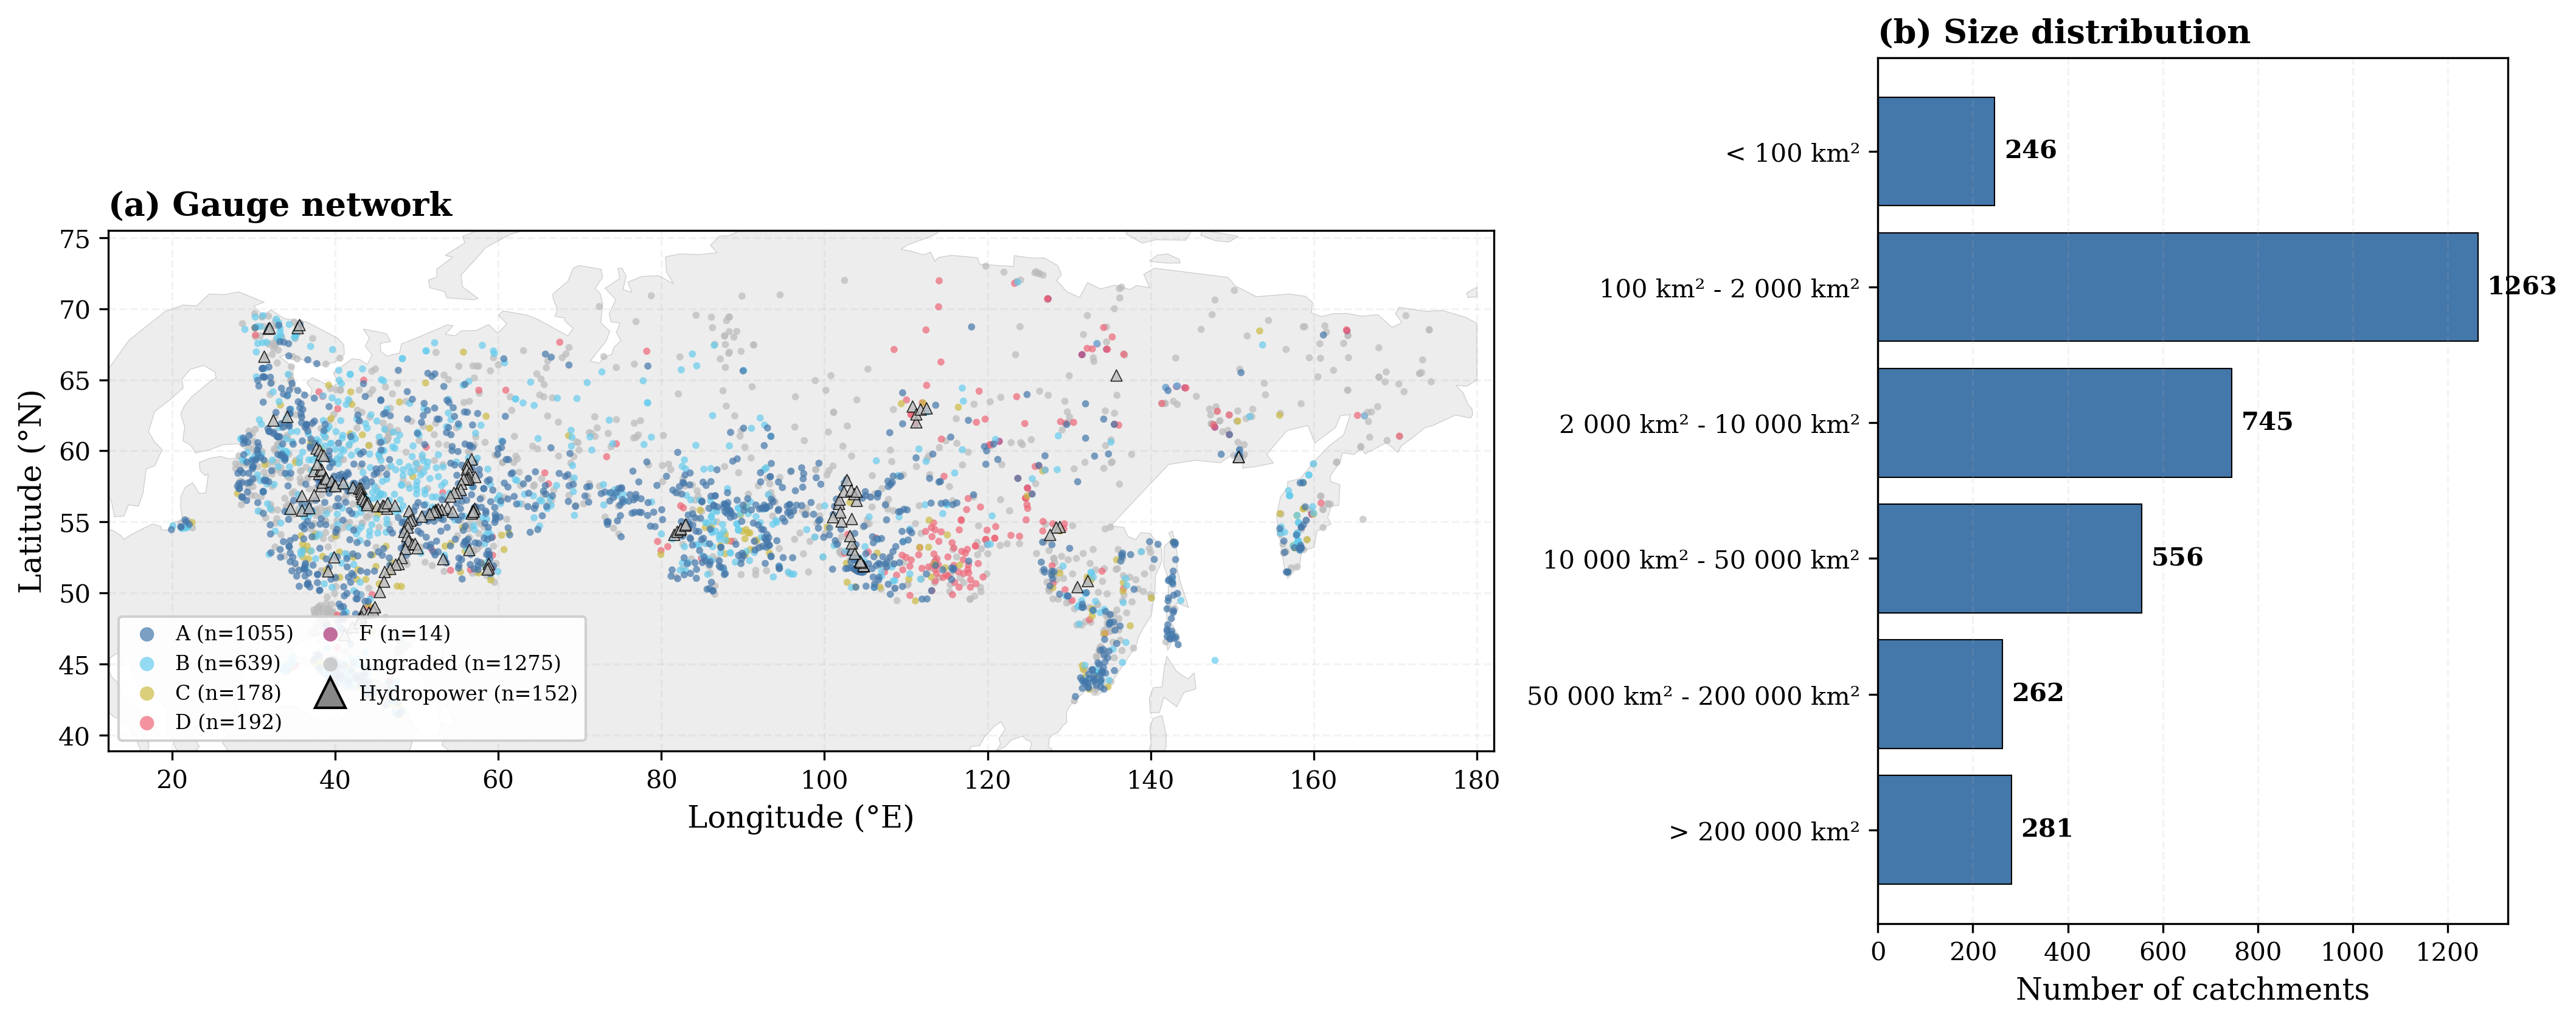
\includegraphics[width=0.95\columnwidth]{../images/fig_gauge_network.png}
\caption{(a) Spatial distribution of \ntotal gauging stations colored by discharge quality grade (A--F; triangles denote hydropower stations). (b) Catchment size distribution. Higher gauge density in European Russia and southern Siberia reflects Roshydromet's operational network.}
\label{fig:gauge_network}
\end{figure}
